%---------------------------------------------------------------------
%	个性化信息
%--------------------------------------------------------------------
\newcommand{\MYTITLE}{污秽之世,美丽之笼}%论文标题
\newcommand{\MYID}{2333333}%学号
\newcommand{\MYNAME}{博丽灵梦}%姓名
\newcommand{\MYCLASS}{博丽神社}%班级
\newcommand{\MYADVISOR}{上白泽慧音}%任课教师
\newcommand{\MYCOURSE}{东方永夜抄}%课程名
\newcommand{\MYTERM}{2021年春季学期}%学期
\newcommand{\MYCOURSEID}{233333}%课程ID
%---------------------------------------------------------------------
%   各种导言
%--------------------------------------------------------------------
\documentclass[a4paper,12pt]{report}
\usepackage[margin=1in]{geometry} % to change the page dimensions
\usepackage{ctex}
\usepackage{xeCJK}
\usepackage{comment}
\usepackage{setspace}
\usepackage{fancyhdr}
\usepackage{graphicx}
\usepackage{wrapfig}
\usepackage{subfigure}
\usepackage{array}
\usepackage{titlesec}
\usepackage{titletoc}
\usepackage[titletoc]{appendix}
%\usepackage[top=30mm,bottom=30mm,left=20mm,right=20mm]{geometry}
%\usepackage{cite}

%\usepackage{courier}
\setmonofont{Courier New}
\usepackage{listings}
%---------------------------------------------------------------------
%   参考文献设置
%--------------------------------------------------------------------
\usepackage[backend = biber, style = references/gb7714-2015, defernumbers=true]{biblatex}
\renewcommand*{\bibfont}{\small}
\addbibresource{references/bibtest.bib}
\renewcommand{\bibname}{参考文献}
%---------------------------------------------------------------------
%	引用文献设置为上标
%---------------------------------------------------------------------
\begin{comment}
    \makeatletter
    \def\@cite#1#2{\textsuperscript{[{#1\if@tempswa , #2\fi}]}}
    \makeatother
\end{comment}

\lstset{tabsize=4, keepspaces=true,
    xleftmargin=2em,xrightmargin=0em, aboveskip=0.1em,
    %backgroundcolor=\color{gray!20},  % 定义背景颜色
    frame=none,                       % 表示不要边框
    extendedchars=false,              % 解决代码跨页时,章节标题,页眉等汉字不显示的问题
    numberstyle=\ttfamily,
    basicstyle=\ttfamily,
    keywordstyle=\color{blue}\bfseries,
    breakindent=10pt,
    identifierstyle=,                 % nothing happens
    commentstyle=\color{green}\small,  % 注释的设置
    morecomment=[l][\color{green}]{\#},
    numbers=left,stepnumber=1,numberstyle=\scriptsize,
    showstringspaces=false,
    showspaces=false,
    flexiblecolumns=true,
    breaklines=true, breakautoindent=true,breakindent=4em,
    escapeinside={/*@}{@*/},
}
\usepackage{amsmath}
\usepackage{amsthm}
\newtheorem{theorem}{定理}
\newtheorem{definition}{定义}
\newtheorem{corollary}{推论}
\newtheorem{example}{例}
\renewcommand {\thetable} {\arabic{table}}
\renewcommand {\thefigure} {\arabic{figure}}
\usepackage{amsfonts}
%\usepackage{bm}
\usepackage{booktabs} % for much better looking tables
\usepackage{paralist} % very flexible & customisable lists (eg. enumerate/itemize, etc.)
\usepackage{verbatim} % adds environment for commenting out blocks of text & for better verbatim
\usepackage{subfigure} % make it possible to include more than one captioned figure/table in a single float
% These packages are all incorporated in the memoir class to one degree or another...
\usepackage{cases} %equation set
\usepackage{multirow} %use table
\usepackage{algorithm}
\usepackage{algorithmic}
%\usepackage{cite}
\usepackage{hyperref}
\usepackage{longtable}
\usepackage{caption}
\usepackage{zhnumber} % change section number to chinese
\hypersetup{colorlinks,linkcolor=black,anchorcolor=black,citecolor=black, pdfstartview=FitH,bookmarksnumbered=true,bookmarksopen=true,} % set href in tex & pdf
%\usepackage[framed,numbered,autolinebreaks,useliterate]{mcode} % 插入matlab代码
\XeTeXlinebreaklocale "zh"
\XeTeXlinebreakskip = 0pt plus 1pt minus 0.1pt
\setlength{\baselineskip}{22pt}
%---------------------------------------------------------------------
%	%图标顺序标号,不分章节
%---------------------------------------------------------------------
\usepackage{chngcntr}
\counterwithout{table}{chapter}
\counterwithout{table}{section}
\counterwithout{figure}{chapter}
\counterwithout{figure}{section}
%---------------------------------------------------------------------
%	页眉页脚设置
%---------------------------------------------------------------------
\fancypagestyle{plain}{
    \pagestyle{fancy}      %改变章节首页页眉
}

\pagestyle{fancy}
\lhead{}
\rhead{}
\fancyhead[C]{\MYTITLE}
\cfoot{\thepage}
\renewcommand\thesection{(\zhnum{section})}
\renewcommand \thesubsection {\arabic{subsection}.}
\renewcommand \thechapter {\zhnum{chapter}、}
\titleformat{\chapter}{\centering\zihao{4}\songti\bfseries}{\chinese{chapter}、}{0.05em}{}
\titlespacing{\chapter}{16pt}{16pt}{*6}
\titleformat{\section}{\zihao{-4}\songti\bfseries}{$\qquad$(\chinese{section})}{0.05em}{}
\titleformat{\subsection}{\zihao{-4}\songti\mdseries}{$\qquad$\arabic{subsection}.$\ $}{0.05em}{}

%---------------------------------------------------------------------
%	摘要设置
%---------------------------------------------------------------------
%\renewcommand{\abstractname}{摘要}
\newcommand{\enabstractname}{Abstract}
\newcommand{\cnabstractname}{内容摘要}
\newenvironment{enabstract}{%
  \par\small
  \noindent\mbox{}\hfill{\bfseries \zihao{3} \enabstractname}\hfill\mbox{}\par
  \vskip 2.5ex}{\par\vskip 2.5ex}
\newenvironment{cnabstract}{%
  \par\small
  \noindent\mbox{}\hfill{\bfseries \zihao{3} \cnabstractname}\hfill\mbox{}\par
  \vskip 2.5ex}{\par\vskip 2.5ex}
\renewcommand{\figurename}{图}
\renewcommand{\tablename}{表}



%---------------------------------------------------------------------
%	目录页设置
%---------------------------------------------------------------------
%\renewcommand{\contentsname}{\zihao{-3} 目\quad 录}
\setcounter{tocdepth}{1}
\renewcommand{\contentsname}{\zihao{3}\bfseries\centering{目$\quad$录}}
\titlecontents{chapter}[0em]{\songti\zihao{4}\bfseries}{\thecontentslabel\ }{}
{\hspace{.5em}\titlerule*[4pt]{$\cdot$}\contentspage}
\titlecontents{section}[2em]{\vspace{0.1\baselineskip}\songti\zihao{4}}{\thecontentslabel\ }{}
{\hspace{.5em}\titlerule*[4pt]{$\cdot$}\contentspage}
%\titlecontents{subsection}[4em]{\vspace{0.1\baselineskip}\songti\zihao{-4}}{\thecontentslabel\ }{}
%{\hspace{.5em}\titlerule*[4pt]{$\cdot$}\contentspage}


\begin{document}
%---------------------------------------------------------------------
%	封面设置
%---------------------------------------------------------------------
\begin{titlepage}
    \begin{center}

    
\includegraphics[width=1.0\textwidth]{figure/zhongcai.png}\\
    \vspace{20mm}
    \textbf{\zihao{2}{\heiti\textbf{\MYTITLE}}}\\[0.8cm]
    \vspace{10mm}
    \vspace{\fill}

\setlength{\extrarowheight}{3mm}
{\songti\zihao{3}	
\begin{tabular}{rp{8cm}<{\centering}}
    {\makebox[4\ccwd][s]{学年学期:}} & \kaishu \underline{\makebox[8cm]{\MYTERM}} \\
    {\makebox[4\ccwd][s]{课程名称:}} & \kaishu \underline{\makebox[8cm]{\MYCOURSE}} \\
    {\makebox[4\ccwd][s]{课程代码:}} & \kaishu \underline{\makebox[8cm]{\MYCOURSEID}} \\
    {\makebox[4\ccwd][s]{任课教师:}}  & \kaishu \underline{\makebox[8cm]{\MYADVISOR}} \\
    {\makebox[4\ccwd][s]{班\qquad 级:}} & \kaishu \underline{\makebox[8cm]{\MYCLASS}}  \\
    {\makebox[4\ccwd][s]{学\qquad 号:}} & \kaishu \underline{\makebox[8cm]{\MYID}}  \\
    {\makebox[4\ccwd][s]{姓\qquad 名:}} & \kaishu \underline{\makebox[8cm]{\MYNAME}} \\
    \\
    {\makebox[4\ccwd][s]{总\qquad 分:}} & \kaishu \underline{\makebox[8cm]{}} \\
    {\makebox[4\ccwd][s]{评$\ $分$\ $人:}} & \kaishu \underline{\makebox[8cm]{}} \\
\end{tabular}
 }\\[2cm]
    \end{center}	
\end{titlepage}

%---------------------------------------------------------------------
%  摘要页
%---------------------------------------------------------------------
\begin{cnabstract}
    摘要正文
    \par\textbf{关键字: } 关键字1,关键字2,关键字3
    \end{cnabstract}
    \vspace{10mm}
    \begin{enabstract}
    English abstract
    \par\textbf{Keywords:} keyword1, keyword2, keyword3
    \end{enabstract}
    \thispagestyle{empty}

%---------------------------------------------------------------------
%  目录页
%---------------------------------------------------------------------
\tableofcontents % 生成目录
\thispagestyle{empty}
%---------------------------------------------------------------------
%  引言
%---------------------------------------------------------------------

\chapter*{\zihao{3} \MYTITLE}
\setcounter{page}{1}

这里写引言\cite{王宣承-1}
%---------------------------------------------------------------------
%  正文
%---------------------------------------------------------------------
\chapter{子时一刻}

\begin{table}[h]
    \centering
    \begin{tabular}{lc}
        \toprule[1.5pt]
        成员 & 分工\\
        \midrule[1.0pt]
        博丽灵梦 & 组长、初期报告展示、复制报告汇总\\
        雾雨魔理沙 & 稳健OLS与FGLS回归估计及分地区、年度差异分析\\
        东风谷早苗 & 分位数回归、分地区回归、年度差异分析\\
        十六夜宵夜 & 数据处理、期末汇报展示\\
        魂魄妖梦 & 数据处理、中期报告展示、排版整理\\
        \bottomrule[1.5pt]
    \end{tabular}
\end{table}

\chapter{丑时一刻}
\section{啧啧}
\subsection{阿斯顿}
拆行公式:
\begin{equation*}
\begin{split}
   UNEMSEC = \beta_0 + \beta_1HEA\_0 + \beta_2HEA\_1 + \beta_3OLD\_0 +  \\
     \beta_4OLD\_1 + \beta_5ifiwork + \beta_6family\_income + \epsilon
\end{split}
\end{equation*}

其中,HEA\_0表达是否\footnote{脚注示例}投保基础医疗保险的离散变量,HEA\_1代表是否投保补充医疗保险的离散变量,OLD\_0代表是否投保基础养老保险的离散变量,OLD\_1代表是否投保补充养老保险的虚拟变量,ifiwork代表受访者是否正在就业,family\_income代表家庭总收入.

我们采取logit模型对2006年作为训练集回归,得到模型的预测准确率达到85.36\%.这是可以接受的.随后我们以2015年作为预测集预测了受访者有没有投保失业保险.



\section{慧音}
\subsection{就业情况}
原文中对确定性收入的线性回归解释变量中有“家庭中就业人口比例”这一变量.CGSS2006将有关变量统计在“活动状态”中,具体分为全职就业、半职就业、临时就业、务农、服兵役等14种.考虑到原文希望得到“确定性收入”,我们推测“全职就业”似乎更为贴近“持久就业”的范畴;另外,根据我国《劳动法》的规定:
\begin{quotation}
  \textbf{\zihao{5}就业人口,在我国是指在16周岁以上,特殊职业需要18周岁以上,从事一定社会劳动并获取劳动报酬或经营收入的人员,其中,城镇就业人口是指在城镇地区从事非农业活动的就业人口,包括在国有单位、城镇集体单位、股份合作单位、联营单位、有限责任公司、股份有限公司、私营企业、港澳台投资单位、外商投资单位和个体工商户从业的人员.}
\end{quotation}

据此,我们认为务农、服兵役是不符合“就业”范畴的.


\section{线性回归计算peincome、unincome}
\subsection{被解释变量的选择}
关于这两个变量,原文的描述是:
\begin{quotation}
  \zihao{5}参照前人的方法(Dynan et al. ,2004;罗楚亮,2004),以城镇家庭的\textbf{人均实际收入}作为因变量,选择家庭成员的平均年龄、平均受教育程度、户主的性别和政治面貌、家庭中的就业人口比例以及所在省份等作为自变量进行OLS回归,并使用该方程\textbf{预测值}和\textbf{残差}作为家庭的持久收入和不确定收入.
\end{quotation}

据此我们根据回归方程:表\ref{hhh}

\[
Ave\_income = \beta_0 + \beta_{1}Ave\_age + \beta_{2}Ave\_edu + \beta_{3}hgender + \beta_{4}hccp + \beta_{5}worker\_ratio + \epsilon
\]


\subsection{解释变量的选择}
\subsection{啊啊阿发}
\begin{table}
    \caption{手动插入表格示例1}
    \centering
    \begin{tabular}{lcccc}
        \toprule[1.5pt]
        variable & mean & sd & min & max \\ 
        \midrule[1.0pt]
        SR1 & 0.60 & 0.52 & -5.00 & 1.00 \\ 
        SR2 & 0.47 & 0.63 & -5.38 & 1.00 \\ 
        peincome & 9.72 & 0.60 & 7.86 & 11.92 \\ 
        unincome & 0.00 & 0.74 & -3.35 & 3.71 \\ 
        PENSION & 0.78 & 0.42 & 0.00 & 1.00 \\ 
        HEASEC & 0.93 & 0.26 & 0.00 & 1.00 \\ 
        UNEMSEC & 0.45 & 0.50 & 0.00 & 1.00 \\ 
        r & 0.61 & 0.27 & 0.00 & 1.00 \\ 
        pension & 0.47 & 0.34 & 0.00 & 1.00 \\ 
        heasec & 0.57 & 0.30 & 0.00 & 1.00 \\ 
        unemsec & 0.29 & 0.35 & 0.00 & 1.00 \\ 
        \bottomrule[1.5pt]
    \end{tabular}
\end{table}




\chapter{寅时一刻}
\section{曾依藉的绿}
\begin{figure}[H]
    \centering
    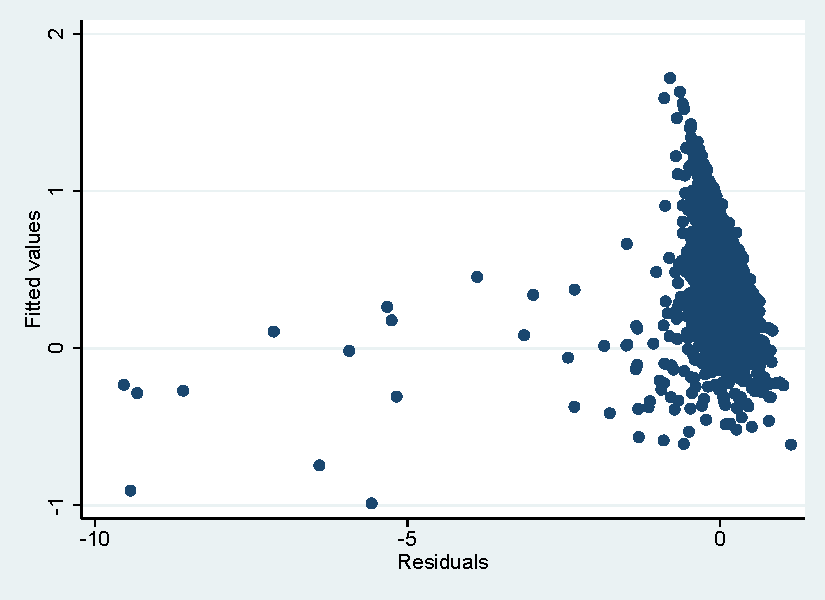
\includegraphics[width=0.65\textwidth]{figure/cancha.pdf}
    \caption{插入图片示例}
\end{figure}

\begin{table}
    \caption{手动插入表格示例2}
    \centering
    \begin{tabular}{lcccc}
        \toprule[1.5pt]
        variable & mean & sd & min & max \\ 
        \midrule[1.0pt]
        SR1 & 0.60 & 0.52 & -5.00 & 1.00 \\ 
        SR2 & 0.47 & 0.63 & -5.38 & 1.00 \\ 
        peincome & 9.72 & 0.60 & 7.86 & 11.92 \\ 
        unincome & 0.00 & 0.74 & -3.35 & 3.71 \\ 
        PENSION & 0.78 & 0.42 & 0.00 & 1.00 \\ 
        HEASEC & 0.93 & 0.26 & 0.00 & 1.00 \\ 
        UNEMSEC & 0.45 & 0.50 & 0.00 & 1.00 \\ 
        r & 0.61 & 0.27 & 0.00 & 1.00 \\ 
        pension & 0.47 & 0.34 & 0.00 & 1.00 \\ 
        heasec & 0.57 & 0.30 & 0.00 & 1.00 \\ 
        unemsec & 0.29 & 0.35 & 0.00 & 1.00 \\ 
        hgender & 0.99 & 0.11 & 0.00 & 1.00 \\ 
        hccp & 0.24 & 0.43 & 0.00 & 1.00 \\ 
        hedu1 & 0.19 & 0.39 & 0.00 & 1.00 \\ 
        hedu2 & 0.32 & 0.47 & 0.00 & 1.00 \\ 
        hedu3 & 0.26 & 0.44 & 0.00 & 1.00 \\ 
        hedu4 & 0.23 & 0.42 & 0.00 & 1.00 \\ 
        headage & 52.50 & 14.95 & 22.00 & 94.00 \\ 
        headage2 & 0.30 & 0.16 & 0.05 & 0.88 \\ 
        rchild1 & 0.03 & 0.09 & 0.00 & 0.67 \\ 
        rchild2 & 0.04 & 0.10 & 0.00 & 0.67 \\ 
        rchild3 & 0.02 & 0.07 & 0.00 & 0.50 \\ 
        rchild4 & 0.02 & 0.08 & 0.00 & 0.67 \\ 
        rchild5 & 0.02 & 0.08 & 0.00 & 0.50 \\ 
        rold & 0.21 & 0.36 & 0.00 & 1.00 \\ 
        ln\_ha & 3.44 & 0.66 & 0.18 & 6.11 \\ 
        \bottomrule[1.5pt]
    \end{tabular}
    \label{hhh}
\end{table}


插入代码示例:
\begin{lstlisting}[language=C]
    qui reg SR1 $xx dummy1-dummy24 if time==0
    predict e1,res
    g e2 = e1^2
    g lne2 = log(e2)
    qui reg lne2 peincome if time==0,noc
    predict lne2f
    g e2f =exp(lne2f)
    reg SR1 $xx dummy1-dummy24 if time==0 [aw=1/e2f]
\end{lstlisting}


%---------------------------------------------------------------------
%  参考文献
%---------------------------------------------------------------------
\printbibliography

\end{document} 
